\documentclass{beamer}
\usetheme{Warsaw}

\usepackage{xcolor}
\usepackage{amsmath, amssymb, amsfonts, amsthm, amssymb}
\usepackage{url, hyperref}

% Usar plantilla en español.
\usepackage[spanish]{babel}

% Agregar citas bibliográficas
\usepackage{cite}

% Poner código fuente en latex
\usepackage{listings}
\usepackage{color}

\usepackage{listings}
\usepackage{booktabs}
\usepackage{bookmark}
\usepackage{makecell}
\usepackage{url}
\usepackage{multirow}
\usepackage{graphicx}

\usepackage{beamerthemesplit}

\definecolor{gray97}{gray}{.97}
\definecolor{gray75}{gray}{.75}
\definecolor{gray45}{gray}{.45}


\title[Moogle!]{\LARGE Moogle!}
\author{Eduardo Brito Labrada}
\institute[Universidad de La Habana]
{
  Facultad de Matem\'atica y Computaci\'on
}
\date{\today}

\begin{document}
\begin{frame}
\maketitle
\end{frame}

\section{Una breve introducci\'on}

\begin{frame}{Una breve introducci\'on}
  \begin{center}
    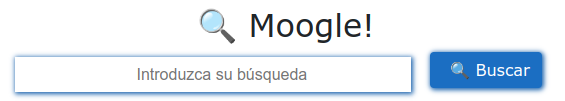
\includegraphics[width=10cm]{images/moogle.png}
  \end{center}

  Moogle! es una aplicación {\em totalmente original} cuyo propósito es buscar
  inteligentemente un texto en un conjunto de documentos.
\end{frame}

\begin{frame}{Una breve introducci\'on}
  Es una aplicación web, desarrollada con tecnología {\tt .NET Core 6.0}, específicamente
  usando Blazor como {\it framework} web para la interfaz gráfica, y en el
  lenguaje {\tt C\#}. \\
\end{frame}

\begin{frame}{Una breve introducci\'on}

  La aplicación está dividida en dos componentes fundamentales:

  \begin{itemize}[<+->]
    \item {\tt MoogleServer} es un servidor web que renderiza la interfaz gráfica y sirve los resultados.
    \item {\tt MoogleEngine} es una biblioteca de clases donde está\dots ehem\dots casi implementada la lógica del algoritmo de búsqueda.
  \end{itemize}
\end{frame}

\subsection{?`Para qu\'e sirve?}

\begin{frame}{?`Para qu\'e sirve?}
  La idea original del proyecto es buscar en un conjunto de archivos de texto
  (con extensión {\tt \color{gray45} .txt}) que estén en la carpeta {\tt
      \color{gray45}Content}.
\end{frame}

\subsection*{?`C\'omo usarlo?}

\begin{frame}
  Primeramente, se aconseja a quien use esta aplicaci\'on tener instalado
  \href{https://es.wikipedia.org/wiki/Linux}{Linux}, ya que no se garantiza la
  misma eficiencia si esta en un dispositivo que use Windows.
\end{frame}

\begin{frame}
  En caso de tener instalado Windows, puede optar por
  \href{https://learn.microsoft.com/es-es/windows/wsl/install}{instalar Windows
    Subsystem for Linux (WSL)} que a\~nade funcionalidades de Linux en Windows.
\end{frame}

\subsubsection*{Instrucciones}

\begin{frame}{Instrucciones}
  Lo primero que el usuario debe hacer para poder usar este proyecto es
  \href{https://learn.microsoft.com/es-es/dotnet/core/install/}{instalar {\tt
        .NET Core 6.0}}.

  \pause

  Luego, debe pararse en la carpeta del proyecto y dependiendo de su sistema
  operativo hacer lo siguiente:

  \begin{itemize}[<+->]
    \item {\bf Linux o WSL:} Debe tener instalado {\tt make}. Puede instalarlo ejecutando el siguiente comando en el terminal {\tt sudo apt update \&\& sudo apt install make}. Luego deber\'a ejecutar {\tt make dev}
    \item {\bf Windows:}  Debería poder ejecutar este proyecto usando {\tt dotnet watch run --project MoogleServer}
  \end{itemize}
\end{frame}

\begin{frame}{Instrucciones}
  \begin{itemize}
    \item Abra en su navegador \href{http://localhost:5000}{http://localhost:5000}
    \item Introduzca su b\'usqueda en la ``entrada'' y luego presionando el bot\'on
          ``Buscar''
  \end{itemize}
\end{frame}

\section*{Motor de b\'usqueda}

\begin{frame}{Motor de b\'usqueda}
  El motor de búsqueda usa un modelo vectorial que computa para una {\it query}
  dada qué tan relevante es un documento determinado.
\end{frame}

\begin{frame}{Motor de b\'usqueda}
  Este modelo vectorial usa
    {\it TF-IDF} con {\it Cosine
      Similarity} para computar la relevancia.
\end{frame}

\subsection*{TF-IDF}

\begin{frame}{Term Frequency and Inverse Document Frequency}
  Para computar el vector {\it TF-IDF}
  se hace uso de la fórmula:

  \begin{equation}
    TFIDF = (\frac{tf}{tw}) \times \ln(\frac{td}{dt}) \nonumber
  \end{equation}

  \begin{itemize}
    \item $tf$ es la frecuencia del término en el documento actual.
    \item $tw$ es la cantidad de palabras totales en el documento actual.
    \item $td$ es la cantidad total de documentos a analizar.
    \item $dt$ es la cantidad de documentos que contienen el término.
  \end{itemize}

  \pause

  {\bf \color{red} Nota:} dado que $\frac{td}{dt}$ puede causar problemas por la
  división entre $0$ decidí que si $dt = 0$ luego $TFIDF = 0$, tiene sentido hacer esto ya
  que si $dt = 0$ el término no aparece en ningún documento.
\end{frame}

\subsection*{Cosine Similarity}

\begin{frame}{Cosine Similarity}
  \begin{columns}[T]
    \begin{column}[T]{6cm}
      Después de lo anterior necesitamos calcular la ``similitud'' entre el
      vector {\it document} y el vector {\it query} para lo cual se hace uso de {\it
          Cosine Similarity}.
    \end{column}
    \begin{column}[T]{5cm}
      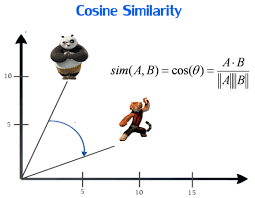
\includegraphics[width=5cm]{images/cosine.png}
    \end{column}
  \end{columns}
\end{frame}

\begin{frame}{Cosine Similarity}
  La idea es intentar estimar el ``ángulo'' comprendido entre
  el vector {\it query} y el vector {\it document}: mientras menor sea este
  ángulo, mayor ``similitud'' tendrán estos vectores. Para lo anterior se hace
  uso de la f\'ormula:

  \begin{equation}
    \cos \alpha = \frac{v_d \cdot v_q}{||v_d|| ~ ||v_q||} \nonumber
  \end{equation}

  \begin{itemize}
    \item $v_d$ el vector de {\it document}
    \item $v_q$ el vector de {\it query}
    \item $||v||$ es la magnitud del vector $v$
  \end{itemize}
\end{frame}

\section{Funcionalidades adicionales}

\begin{frame}{Funcionalidades adicionales}
  Están implementados y se pueden usar sin problemas de ningún tipo los siguientes operadores:

  \begin{itemize}[<+->]
    \item $!$: delante de una palabra este símbolo indica que esa palabra {\bf no debe aparecer} en ningún documento que sea devuelto.
    \item $\wedge $: delante de una palabra este símbolo indica que esa palabra {\bf debe aparecer} en cualquier documento que sea devuelto.
    \item $\sim$: entre dos o más términos este símbolo indica que esos términos deben aparecer cerca, o sea, que mientras más cercanos estén en el documento mayor será la relevancia.
    \item $*$: cualquier cantidad de símbolos $*$ delante de un término indican que ese término es más importante, por lo que su influencia en el {\tt score} debe ser mayor que la tendría normalmente (este efecto será acumulativo por cada $*$)
  \end{itemize}
\end{frame}

\end{document}